\documentclass[a4paper, 12pt]{report}

\pagestyle{empty}

\usepackage{tikz}
\usetikzlibrary{knots}


\begin{document}

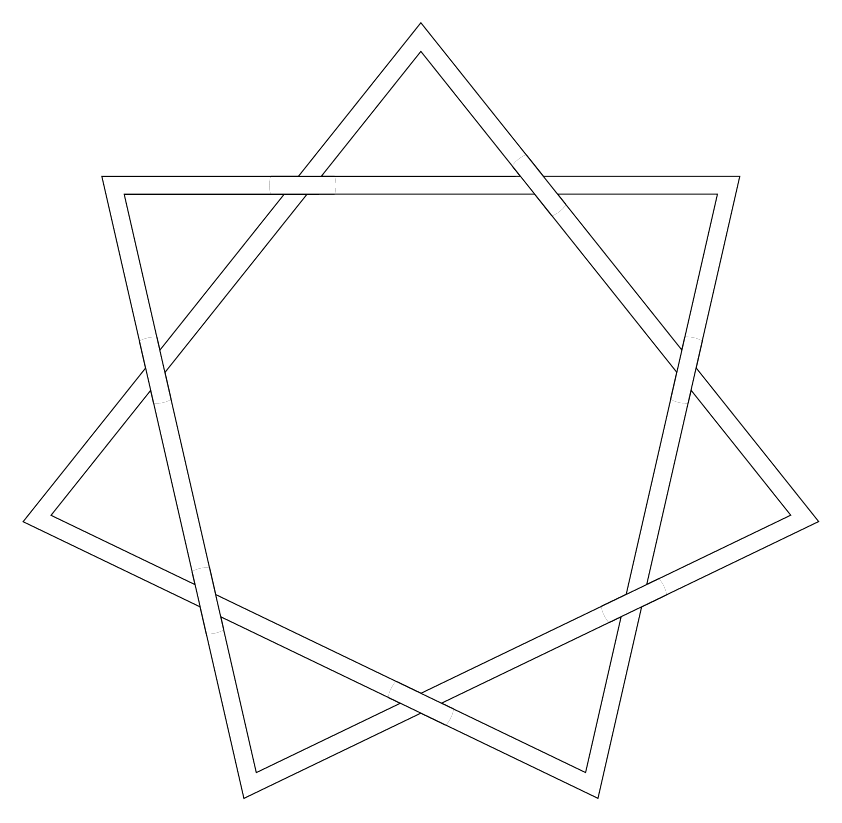
\begin{tikzpicture}
\def\R{5} % Radius of the pentagram
\def\nbre{7} % To define a pentagram --> 7 = heptagram etc.
\pgfmathsetmacro\nbremo{\nbre-1}
\def\decalage{2} % nbre mod decalage != 0

\begin{knot}[
%draft mode = crossings,
%flip crossing/.list = {}, % Format {a,b}
consider self intersections = true,
only when rendering/.style = {black, double, double distance = 6pt}
%only when rendering/.style = {white, line width = 3pt, double = black, double distance = 6pt}
]
%\strand (90:\R) -- (-54:\R) -- (162:\R) -- (18:\R) -- (-126:\R) -- (90:\R) -- cycle;
% VS
%\strand (90:\R) -- (-54:\R) -- (162:\R) -- (18:\R) -- (-126:\R) -- cycle;
\flipcrossings{2,4} % nbre = 5

\strand (90:\R) \foreach \k in {1,...,\nbremo} {-- (90 - \decalage/\nbre*\k*360:\R)} -- cycle; % Automated path
% !!! AJUSTER les flip crossing manuellement !!!
\end{knot}
\end{tikzpicture}

\end{document}
